\newpage
\section{Use cases}
To get an overview of the system functionality from a user's perspective, the team applied \glspl{usecase}. This is a technique to help developers identify functionality that should be implemented, and possible errors that might occur in the system.

The primary actor in this system is the Android app user. An example use case diagram of the final version of the system is shown in figure~\ref{fig:usecase}. For an overview of all textual use cases, see Appendix~\ref{sec:textUseCase}.\\

\begin{figure}[H]
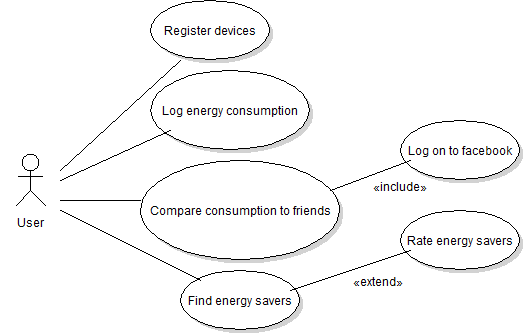
\includegraphics[width=\textwidth]{ch/specification/fig/currentUsecase.png}
\caption{Example use case diagram for the system}
\label{fig:usecase}
\end{figure}
